We consider the problem of reasoning over unstructured contexts in this chapter, and propose to build a model that can jointly retrieve and
reason over them.

\section{Memory Networks}
%TODO: General introduction about the need for explicit memory.
Memory Networks (MemNet) are a class of models
that combine inference with long-term memory. Unlike Recurrent Neural Networks
(RNN) that model language \citep{mikolov2010recurrent}, and their variants with
Long Short-Term Memory (LSTM) \citep{hochreiter1997long}, MemNets have an explicit
memory component with read and write functions. While the original MemNet model 
proposed by \cite{weston2014memory}, MemNN required explicit supervision
for selecting the relevant parts of the memory, \citep{sukhbaatar2015end}
proposed a end-to-end variant (MemN2N) where the memory selection component is
trained jointly with the rest of the network. These were previously used for
answering questions that require reasoning over multiple context sentences,
both in simulated \citep{bordes2010towards} and large-scale
\citep{fader2013paraphrase} scenarios.

In this chapter, we use the term \textit{memory network},
or the abbreviation \textit{MemNet}, to refer to any neural network model with an explicit memory component
that can be read from or written to. Our focus is mostly on the general class of models. Wherever necessary,
we refer to the original memory network model
proposed by \cite{weston2014memory} as \textit{MemNN} and the end to end model by \cite{sukhbaatar2015end}
as MemN2N.


\begin{figure*}
\begin{center}
  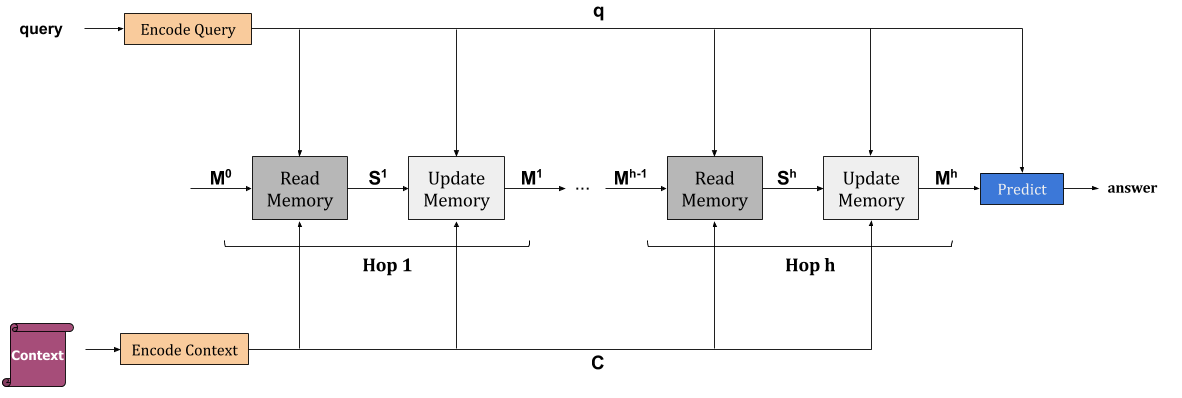
\includegraphics[width=7in]{figures/memory_network_generic.png}
  \caption{Schematic showing a generic view of memory networks}
  \label{fig:memnet}
  \end{center}
\end{figure*}
Figure~\ref{fig:memnet} shows the setup of a generic MemNet. It
takes as inputs:
\begin{itemize}
 \item a set of $N$ context sentences, indexed as $\{context_i\}_{i=1}^N$,
such that $context_i$ is a vector containing the indices of words in the $i^\text{th}$ sentence.
  \item a query, a single sentence indexed similar to context.
\end{itemize}

The sentences are then encoded using the \texttt{EncodeContext} and \texttt{EncodeQuery}
functions to produce the matrix $\textbf{C}$ and $\textbf{q}$ respectively.

The memory network then reasons over the context, represented \textbf{C}, given the 
query, represented by \textbf{q} over multiple memory layers, corresponding to multiple hops $i \in \{1, \ldots, h\}$.
At each hop, a memory layer performs two actions:
\begin{itemize}
 \item \texttt{ReadMemory} gets as input either the context ($\textbf{C}$) (in the first hop) or an updated memory representation ($\textbf{M}^i$)
 (in subsequent hops), and the query representation ($\textbf{q}$) to produce a summary of the memory $\textbf{S}^{i+1}$.
 \item \texttt{UpdateMemory} produces an updated memory representation ($\textbf{M}^{i+1}$) given the summary ($\textbf{S}^i$) and the query ($\textbf{q}$).
\end{itemize}

Finally, an answer is
predicted by passing the query encoding $\textbf{q}$, and the memory state at the
last hop ($\textbf{M}^h$) to the \texttt{Predict} function.

It can be seen that MemN2N fits into this setup with the following
configuration:
\begin{flalign}
&\texttt{EncodeQuery}(\text{query}) = \text{BOWEncoder}_q(\text{query}) \in \mathbb{R}^{d}\\
&\texttt{EncodeContext}(\text{Context}) = \text{BOWEncoder}_c(\text{Context}) \in \mathbb{R}^{N \times d}\\
&\texttt{ReadMemory}(\textbf{q}, \textbf{M}^{i-1}, \textbf{C}) = \text{softmax}(\textbf{C}.\textbf{M}^{i-1}).\textbf{C} \in \mathbb{R}^d\\
&\texttt{UpdateMemory}(\textbf{q}, \textbf{S}^i, \textbf{C}) = \textbf{q} + \textbf{S}^i \in \mathbb{R}^d \\
&\texttt{Predict}(\textbf{q}, \textbf{M}^h) = \text{softmax}(W.\textbf{M}^h) \in \mathbb{R}^o
\end{flalign}

where $\text{BOWEncoder}_q(.)$ and $\text{BOWEncoder}_c(.)$ are simply bag of
words models that aggregate the vector representations of all the words given by
the indices in the input and average them. $W \in \mathbb{R}^{o \times d}$ is a parameter of the
answer prediction function, causing the softmax to be over the output vocabulary size
$o$. Note that in MemN2N, \textbf{q} is not used in \texttt{ReadMemory} and \texttt{Predict}, and
\textbf{C} is not used in \texttt{UpdateMemory} since MemN2N is one of the simplest forms of MemNets.

In contrast, Gated Attention Reader \cite{dhingra2016gated} is relatively more complex, and uses the following
configuration:

\begin{flalign}
&\texttt{EncodeQuery}(\text{query}) = \text{Bi-GRU}_q(\text{query}) \in \mathbb{R}^d\\
&\texttt{EncodeContext}(\text{Context}) = \text{Bi-GRU}_c(\text{Context}) \in \mathbb{R}^{N_w \times d}\\
&\texttt{ReadMemory}(\textbf{q}, \textbf{M}^{i-1}, \textbf{C}) = \text{softmax}(\textbf{M}^{i-1}.\textbf{q}).\textbf{M}^{i-1} \in \mathbb{R}^{N_w \times d}\\
&\texttt{UpdateMemory}(\textbf{q}, \textbf{S}^i, \textbf{C}) = \text{Bi-GRU}_c(\textbf{S}^i.\textbf{q}) \in \mathbb{R}^{N_w \times d} \\
&\texttt{Predict}(\textbf{q}, \textbf{M}^h) = \text{softmax}(\textbf{M}^h.q) \in \mathbb{R}^{N_w}
\end{flalign}

The encoders used here are bidirectional Recurrent Neural Networks with Gated Recurrent Units \cite{cho2014learning}. Note that the output of $\text{Bi-GRU}_c$
is a matrix because it returns outputs from all time steps as a sequence. $N_w$ here denotes the number of tokens in all $N$ sentences in context. The output
produced here is a probability distribution over all tokens in the context, because this model was proposed for tasks that involve directly selecting a token from
the context.

Both the models described here assume that the context is well defined and small enough to fit in memory.
In this chapter, we focus on problems where these assumptions do not hold true, and where the context
be retrieved from a big corpus. Accordingly, we propose to add an additional
\texttt{RetrieveContext} module to our generic MemNet architecture.
Particularly, we are interested in developing MemNet models that
can figure out whether the available context is sufficient to make a prediction. We first
describe a target dataset for our model, and then list the issues we propose to address.

\section{Retrieval for Question Answering}
The datasets we use here are significantly different from the
QA datasets previously used to test memory networks, and require more complex
reasoning. One example of such question is shown below.
%TODO(pradeep): Make this a table?
\begin{itemize}
\item Astronauts weigh more on Earth than they do on the moon because
\begin{enumerate}[(a)]
 \item they have less mass on the moon
 \item their density decreases on the moon
 \item the moon has less gravity than Earth
 \item the moon has less friction than Earth
\end{enumerate}
\end{itemize}
%TODO(pradeep): Say more things about the nature of the problem.
The text relevant to questions like this may contain a single sentence that
has the information to answer this question, like this:
\begin{itemize}
 \item People weigh more on some planets than others because of differences in gravity.
\end{itemize}

Or it may span multiple sentences like this:
\begin{itemize}
 \item Moon's gravity is less than that of Earth.
 \item Weight of a person depends on the gravity of the planet.
\end{itemize}

Or in other cases, the text may not contain the relevant answer at all. Hence, this setup
requires a module in addition to the ones mentioned, that retrieves relevant content from
the corpus. However, as the size of the context increases, it becomes more and more expensive to reason over
it. Also, increased context size may add noise to prediction process. Hence, it is important to
retrieve context conservatively, and the model should reason whether the retrieved context
is sufficient to produce an answer.

\paragraph{Question Answering as Textual Entailment} In our proposed setup, we
cast the problem of deciding whether the given context is sufficient to answer the question, as a
textual entailment problem. That is, given a multiple choice question with answer options, we
convert the combination of the question and each of the options into a
statement, and check whether the statement can be entailed from relevant
background information. Given this setup, the \texttt{Predict} function
essentially becomes an entailment function. If none of the question-option combinations
can be entailed from (or contradicted by) the retrieved context, we retrieve more context.

\subsection{Proposed Algorithm}
Based on the ideas described so far, we now present the proposed algorithm, \textsc{AdaptiveRead}
to read and reason, while choosing to retrieve or predict depending on the sufficiency
of the context available.

\begin{algorithm}[H]
 \KwIn{$L$: large corpus, $q$: question}
 \KwOut{$a$: answer}
 $ContextSize = k$ \;
 $C = \texttt{RetrieveContext}(q, L, ContextSize)$, the top $k$ relevant sentences from the corpus\;
 \While{$ContextSize < MaxContextSize$} {
  \eIf{$\texttt{EntailsOrContradicts}(C, q)$}{
    $a = \texttt{Predict}(C, q)$ \;
    return $a$
  }{
    $ContextSize += k$ \;
    $C = \texttt{RetrieveContext}(q, L, ContextSize)$ \;
  }
 }
 \caption{\textsc{AdaptiveRead} algorithm that learns when to stop retrieving context}
\end{algorithm}

This algorithm shares some similarities with the \textit{ReasoNet} model
proposed by \cite{shen2016reasonet}, but the main difference is that while ReasoNet learns to
stop performing additional hops, the proposed algorithm learns to stop retrieving additional context.

\subsection{Potential Issues}
We identify the following potential issues in building \textsc{AdaptiveRead}.
\begin{enumerate}
 \item \textbf{Scalability to large corpora}: Depending on the complexity of \texttt{ReadMemory}, reasoning
 over large corpora may prove to be intractable. Earlier work in solving this problem involves building
 hierarchical models \citep{chandar2016hierarchical,choi2016hierarchical}. While \cite{chandar2016hierarchical}
 build a hierarchical memory network that uses a simple dot product for \texttt{RetrieveContext} and \texttt{ReadMemory},
 and thus use maximum inner product search (MIPS) to do them efficiently, \cite{choi2016hierarchical} perform summarization
 to retrieve context followed by answer prediction. We can use some of their ideas to make \texttt{RetrieveContext} a simpler
 process, and \texttt{ReadMemory} a more expensive one.
 
 \item \textbf{Difficulty in training}: Clearly, \textsc{AdaptiveRead} makes a hard choice between retrieving context and
 predicting an answer, thus making it impossible to train the model end-to-end using back-propagation. \cite{shen2016reasonet}
 and \cite{choi2016hierarchical} get around similar problems that involve hard choices by training with 
 REINFORCE \citep{williams1992simple} algorithm. However, REINFORCE is known to be unstable due to high variance induced by
 sampling.
\end{enumerate}


% \subsection{Preliminary Results}
% We performed some preliminary experiments to understand the 
% We now show some preliminary results of our memory network implementation on science question answering using MemN2N architecture with following change in configuration:
% \begin{flalign*}
% &\texttt{PredictAnswer}(u_0, s^H) = \texttt{HeuristicMatch}(u_0, s_h)
% \end{flalign*}
% where \texttt{HeuristicMatch}(.) is the heuristic matching function proposed by \cite{mou2015recognizing} for textual entailment, also used for our experiments with SNLI data in 
% Chapter~\ref{chapter:ontolstm}. The dataset used for these experiments is questions collected from 4th and 8th grade science text books.
% Context for each question was obtained as follows. We built a Lucene index over a big collection of sentences related to general science from various sources and extracted relevant background sentences for each question by querying it. For each of the
% options, we query the Lucene index with a combination of the option text and the question. We thus transform questions like the one shown above into four entailment problems where the combination of the
% question and one of the options is the hypothesis and the relevant background sentences are the premises. The final answer is picked by selecting the option (combined with the question) that has the highest
% entailment score. This is done by passing the final entailment scores through a softmax layer.
% 
% Preliminary results using our model are shown in Table~\ref{tab:memnet_qa_results}, using two different encoders
% to encode the input sentences and background. We also show the accuracy of a baseline system based on Lucene, that selects for every question, the option that results in the highest relevance score in the process
% described above for retrieving background sentences. It can be seen that the simple baseline does better than the memory network model.
% 
% \begin{table}
%     \centering
%     \begin{tabular}{|l|c|}
%     \hline
%     \textbf{Encoder} & \textbf{Test Acc.}\\
%     \hline
%     BOW & \% \\
%     GRU & 38.8\% \\
%     \hline
%     \hline
%     \textbf{Lucene baseline} & 41.1\% \\
%     \hline
%     \end{tabular}
%     \caption{Results of our Memory Network on ScienceQA in comparison with a Lucene baseline}
%     \label{tab:memnet_qa_results}
% \end{table}
% 
% \subsection{Analysis}
% 
% \subsection{Proposed Work}


